\pagestyle{empty}
\chapter*{\centering \large DAFTAR RIWAYAT HIDUP}
\thispagestyle{empty}
\onehalfspacing{}

\begin{wrapfigure}[6]{l}{4cm}
	\vspace{-25pt}
	\begin{center}
		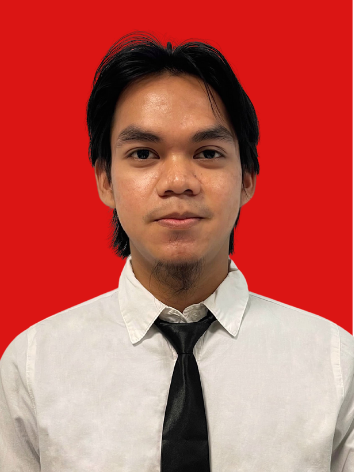
\includegraphics[width=0.27\textwidth]{gambar/pas_foto/ridho}
	\end{center}
	\vspace{-40pt}
\end{wrapfigure}

\noindent \textbf{MUHAMMAD RIDHO RIZQILLAH}. Lahir di Jakarta, 24 Agustus 2001. Anak ketiga dari pasangan Bapak Sumarsono dan Ibu Siti Haeriyah. Saat ini penulis tinggal di Komplek Pertamina Tugu Jl. Permata III Blok G Nomor 11 RT 002/RW 016, Kelurahan Tugu Utara, Kecamatan Koja, Kota Jakarta Utara, Provinsi DKI Jakarta.

\vspace{2.5cm}
% \noindent
% \begin{tabular}{lcl}
% 	Email	& :&  mridhor08@gmail.com
% \end{tabular}
% \vspace{0.5cm}

\noindent \textbf{Riwayat Pendidikan}: Penulis mengawali pendidikan di SD Negeri Tugu Utara 15 pada tahun 2007-2013. Setelah itu, penulis melanjutkan pendidikan ke SMP Negeri 30 Jakarta pada tahun 2013-2016. Kemudian melanjutkan pendidikan di SMA Negeri 52 Jakarta pada tahun 2016-2019. Pada tahun 2019, penulis melanjutkan studi ke Universitas Negeri Jakarta (UNJ) di program studi Ilmu Komputer.
\vspace{0.5cm}

\noindent \textbf{Riwayat Organisasi}: Selama di bangku perkuliahan, penulis pernah mengikuti organisasi Badan Eksekutif Mahasiswa selama dua periode yakni 2 semester sebagai Staff dan Kepala Departemen Advokasi. Lalu mengikuti organisasi pengabdian masyarakat Desa Binaan selama 2 semester sebagai Kepala Sub Divisi Kurikulum. Serta menjadi bagian dari Tim Pembela Mahasiswa di UNJ selama satu semester sebagai Staff Kajian dan Aksi Strategis. Tidak lupa pula, penulis juga mengikuti DEFAULT, yakni kelompok studi di program studi Ilmu Komputer yang bergerak di bidang pengembangan teknologi seperti pada bidang arsitektur, \emph{website}, animasi, dan juga aplikasi. Dan menjabat selama 2 semester sebagai Ketua \emph{Website Development Study Interest Group}.